\chapter{Estimating $\Omega_\text{b}(\text{BLA})$} \label{ch:Omega-b}

In this chapter we discuss the estimation of the baryon energy density trapped in BLAs, i.e. $\Omega_\text{b}(\text{BLA})$, using our BLA survey which is the cornerstone of the current work. We will statistically estimate the $\Omega_\text{b}(\text{BLA})$ from our survey results. And then we will determine how much BLAs contribute to the baryon budget ($\Omega_\text{b}$) of the current universe.

\section{Methodology to determine $\Omega_\text{b}(\text{BLA})$}

The baryon content of any ion in terms of the current critical density $(\rho_{cr})$ of the universe can be estimated by integrating over the bivariate frequency distribution of the absorbers as function of column density and redshift of that ion and is given as :

\begin{equation} \label{eqn:omega_ion}
    \Omega_{\text{ion}} = \frac{H_0 m_{\text{ion}}}{c \rho_{\text{cr}}} \int \frac{\partial ^2 \mathcal{N}}{\partial N \partial X} N dN 
\end{equation}

\vspace*{3mm}

Where, $H_0$ is the current value of Hubble's constant, \\ \hspace*{19mm}
$m_\text{ion}$ is the the mass of ion, \\ \hspace*{19mm}
$c$ is the speed of light in vacuum, \\ \hspace*{19mm}
$\mathcal{N}$ is the number of absorbers at column density $N$ and path length $X$

\newpage

The path length $X$ is function of redshift (\emph{z}) and denotes the total absorption path length available for absorption. A non-evolving population of absorbers will show an invariant number density per unit absorption pathlength \citep{Becker-2011}. It is defined as :

\begin{equation}
    X(z)=\int_0^z  (1+z')^2 \frac{H_0}{H(z')} dz'
\end{equation}

Now, assuming a flat $\Lambda \text{CDM}$ cosmology, we can write the Hubble's constant at any \emph{z} as :

\begin{equation}
    H(z) = H_0 \left[\Omega_m(1+z)^3+\Omega_\Lambda\right]^{1/2}
\end{equation}

with $\Omega_m=0.31$ and $\Omega_\Lambda=0.69$ (ref). This gives,

\begin{equation}
    X(z)=\int_0^z  \frac{(1+z')^2}{\left[\Omega_m(1+z')^3+\Omega_\Lambda\right]^{1/2}} dz'
\end{equation}

However, whole pathlength of X may not be available for absorption due to the presence of Ly$\alpha$ forest lines, absorption from strong ISM lines and intervening IGM lines also in the spectrum. So, some correction needs to be made to get the unblocked absorption pathlength. To calculate this correction, we have developed an interactive program, where we manually select the wavelength regions showing strong absorption features from the above mentioned lines along each sight line. So we exclude these wavelength regions to calculate the unblocked absorption pathlength.

Now, to get the baryon content of BLAs using equation \ref{eqn:omega_ion}, we can use total Hydrogen column density, N(H), and $m_{ion}=\mu . m_H$, where $\mu$ is the mean atomic mass in a.m.u. and $m_H$ is the mass of Hydrogen atom. We take $\mu=1.32$ for $\text{Y}_\text{He}=0.2446$ \citep{Peimbert-2016} taking in account the Helium abundance in the universe. But N(H) is not a directly observable quantity, instead we can get neutral Hydrogen column density, N(\ion{H}{i}), from observations. So we need the correct for the ionisation of Hydrogen to get N(H) from observable N(\ion{H}{i}). This ionisation correction is not trivial and require number of assumptions.

If the gas is collisionally ionised, then we can estimate the hydrogen ionization fraction, which is the ratio of amount of total hydrogen and neutral hydrogen, in equilibrium using the models given by \citet{Sutherland-1993} which related the ionisation fraction to the temperature of the gas. It gives following relation :

\begin{equation} 
    \log f_H \approx 5.4 \log T - 0.33(\log T)^2 -13.9
\end{equation}

This relation is valid in the temperature regimes of $10^5-10^7$ K. Figure \ref{fig:fH} shows the variation of $f_H$ with $T$ based on above relation . We can use this to convert N(\ion{H}{i}) to N(H). However, we need to note that at densities lower than $n_H < 10^{-5} \ \text{cm}^{-3}$, photoionisation from UV background could result in higher hydrogen ionization fraction. But since we don't have the hydrogen densities in the absorbers, so we could possibly underestimate the $f_H$ in such cases (see \citet{Richter_2020, Fang-2001} for more details). Still, we need the temperature to get the ionisation correction. We could only estimate the temperature where the BLA is aligned with some other ion like \ion{O}{vi}. We have only few such cases. In rest of the cases, where we don't have an estimate of temperature, we use the Doppler width, \emph{b}, of the BLA to estimate the temperature assuming pure thermal broadening. This gives us an upper limit on the temperature of the absorber. Now, $b^2=2kT/m_H$, so $T=(m_H / 2k) b^2 $. 

\begin{figure}[t]
    \centering
    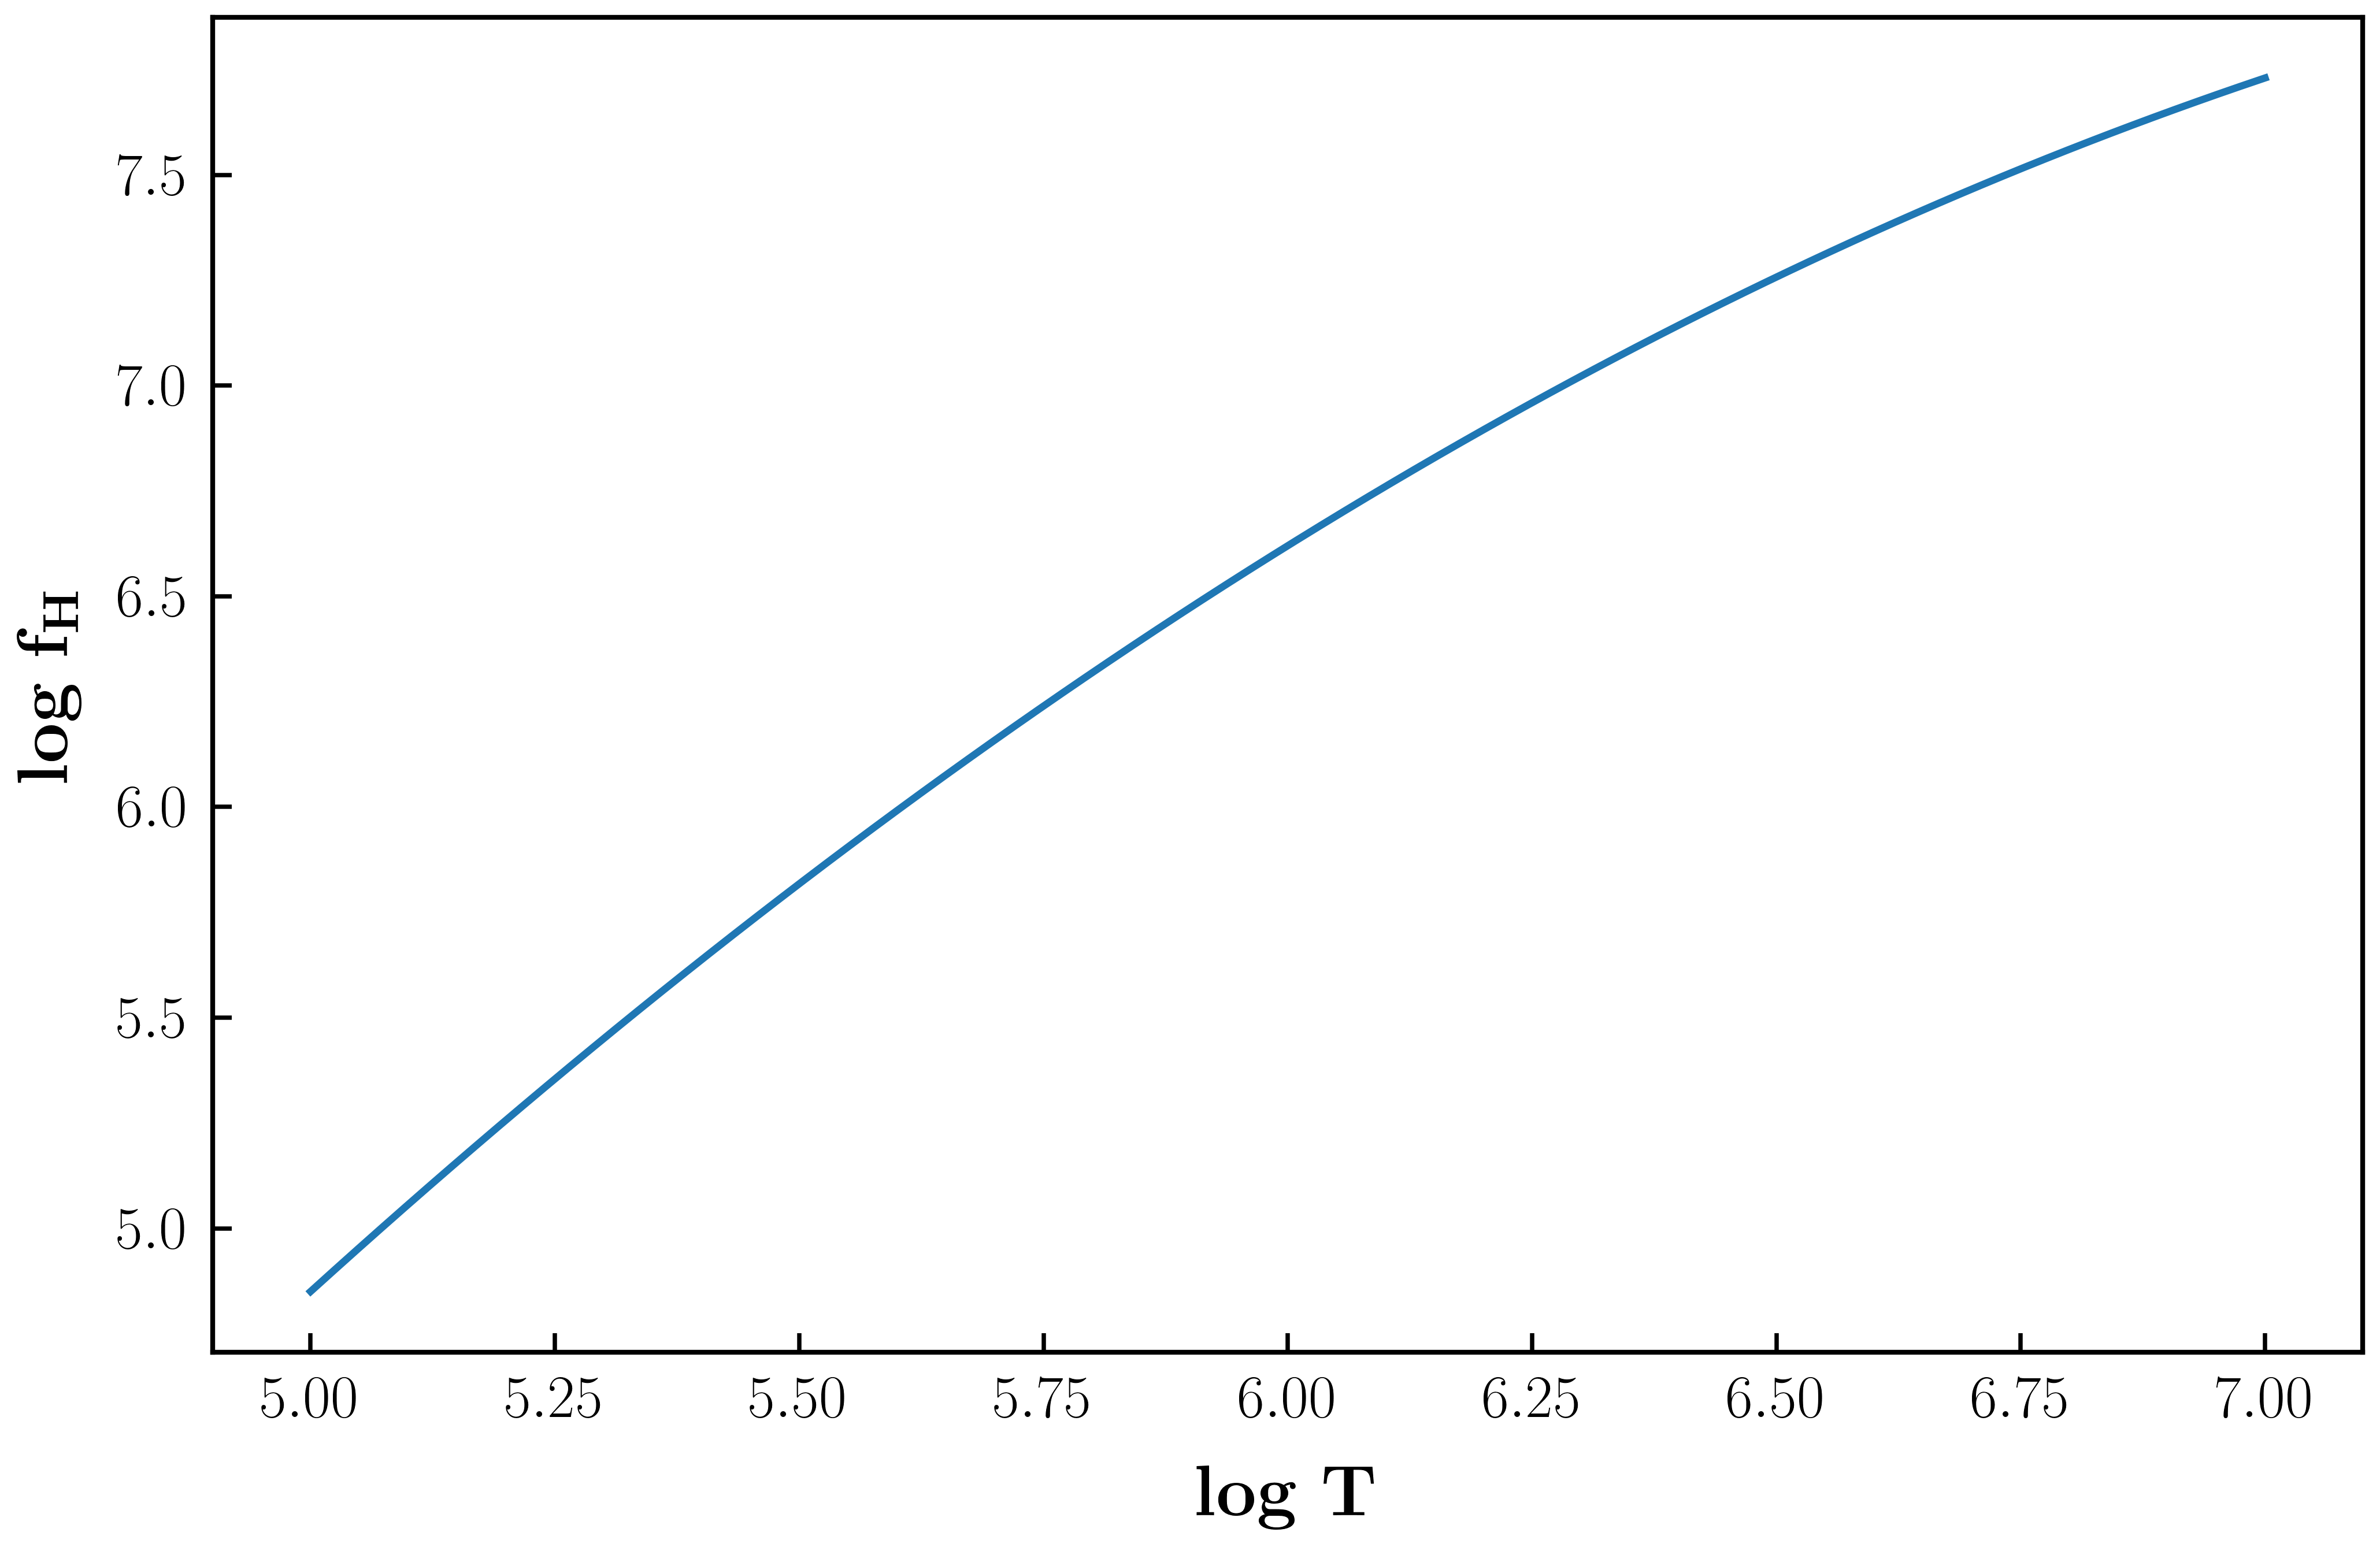
\includegraphics[width=\linewidth]{Figures/fH_vs_T.png}
    \caption{Hydrogen ionisation fraction as a function of temperature.}
    \label{fig:fH}
\end{figure}

Now, as the neutral fraction of hydrogen is very low at the temperatures in WHIM, we can write :

\begin{equation*}
     \log f_H = \log \left(\frac{\ion{H}{i}+\ion{H}{ii}}{\ion{H}{i}}\right) \approx \log \left(\frac{\ion{H}{ii}}{\ion{H}{i}}\right)  \Rightarrow  \ion{H}{ii}= f_H \ion{H}{i}
\end{equation*}

\begin{equation*}
     \Rightarrow  N(\text{H}) = N(\ion{H}{i})+N(\ion{H}{ii}) = (1+f_H)N(\ion{H}{i}) \approx f_H N(\ion{H}{i})
\end{equation*}

Since don;t have the bivariate frequency distribution function, we approximate the intergral in equation \ref{eqn:omega_ion}, which is commonly done, as : 

\begin{equation} \label{eqn:int-approx}
    \int \frac{\partial ^2 \mathcal{N}}{\partial N  \partial X} N dN \simeq \frac{\sum N_{obs}}{\Delta X} 
\end{equation}

Where $N_{obs}$ is the observed column density of the ion and $\Delta X$ is the total unblocked pathlength available. Now using equation \ref{eqn:omega_ion}, the approximation in equation \ref{eqn:int-approx} and including ionisation correction we can estimate $\Omega_\text{b}(\text{BLA})$ as :

\begin{equation}
    \Omega_\text{b}(\text{BLA}) = \frac{H_0 \ \mu m_H}{c \rho_{\text{cr}}} \left. \sum_{i,j} f_{H_{i,j}} N(\ion{H}{i})_{i,j} \ \middle / \sum_j \Delta X_j \right.
\end{equation}

Where $j$ represents a line of sight and $i$ refers to the absorber along sight line $j$. So numerator is the sum over all the absorbers and the denominator is summed over all the lines of sight.  We use error propogation to find the uncertainity in the value of $\Omega_\text{b}(\text{BLA})$. We consider error in $f_H$, which depend on temperature, which inturn depend on the measured \emph{b} values and error in \ion{H}{i} column densities.  

In the next section we describe the sample of absorbers we will be using to estimate the $\Omega_\text{b}(\text{BLA})$.

\section{Selecting the absorber samples}

We have a total of 29 absorber systems in our survey. These systems have 97 \ion{H}{i} components in total. Out of these 97 components, 37(34) components have Doppler parameters above 40(45) km $\text{s}^{-1}$. But as discussed multiple times throughout this work that just having large \emph{b} value does not ensure we have a `true' BLA. So we have to carefully select the candidates which are actually BLAs from these 37(34) components to estimate the baryon content of BLAs. 

\subsection{Based on Temperature and Ionisation Modelling}

Since, we need the temperature to estimate the ionisation fraction, we consider candidates whose temperatures could be estimated from the Doppler parameters of \ion{H}{i} and \ion{O}{vi}. To estimate the temperature directly from Doppler parameters we need that both species must be fairly aligned. HST/COS data may have wavelength calibration errors of 15-20 km s$^{-1}$, which could be as high as few resolution elements \citep{Wakker-2015}. So, we consider species as aligned if they are separated by less 20 km s$^{-1}$ in velocity within the fitting errors. So, if the species are aligned, then we can asssume that they are co-spatial, so that there non-thermal broadening could be assumed to be same. However, we need to be cautious that aligned species need not be co-spatial always. So, upon calculating the temperatures as mentioned.

We get 5 (value) such systems with one-one components each. We call this as sample A and are labelled so in table \ref{tab:CIE-properties}. This sample will give us a conservative lower limit on the baryon content in BLAs. Using this sample of absorbers we get $\Omega_\text{b}(\text{BLA})=0.0018 \pm 0.05$. Table \ref{tab:Omega_b_sampleA} gives the details of the individual sight lines in this sample.  


\subsection{Based on Ionisation Modelling} \label{sec:sampleB}

As discussed in chapter \ref{ch:Survey} we have modelled the ionising conditions in 25 components of 17 \ion{O}{vi} absorbers. And found that 20 of the components could not be explained with photoionisation models, so these could possibly be arising from collisionally ionised gas phase. So these absorbers could potentially be tracing warm hot plasma in WHIM. So we take absorbers where the \ion{O}{vi} could not be explained with photoionisation models and has a broad Ly$\alpha$ line ($\emph{b}>40 \ \text{km s}^{-1}$). We have 14 such systems, which have a total of 21 BLA components. However, we exclude one component towards the sight line of PKS 0637-752 at $z_{comp}=0.161013$ because it has unexpectedly high Doppler parameter of 162 km s$^{-1}$ which affects the estimate of $\Omega_\text{b}(\text{BLA})$ drastically. We get a value of $0.0073 \pm 0.0013$ for $\Omega_\text{b}(\text{BLA})$ using these 20 BLA components. However, if we include the excluded component we get a value of $0.0093 \pm 0.0020$ which is about 27\% higher than the other value. Table \ref{tab:Omega_b_sampleA} gives the details of the individual sight lines in this sample. We could see that individual sight lines have large uncertainities in the $\Omega_\text{b}(\text{BLA})$ value, but the value calculated for whole sample has low uncertainity because of more number of points, hence reducing the statistical errors. 


\begin{longtable}{cccccccc}
            \hline \hline
           \head{$\mathbf{z_{BLA}}$} & \head{\emph{b}} & \head{log N(H \hspace*{-0.5mm}{\footnotesize I})} &  \head{log T}  &  \head{log $\mathbf{f_H}$}  & \head{log N(H)}  & \head{Sample} \tabularnewline
           
             & (km s\textsuperscript{-1}) & (cm\textsuperscript{-2}) & (K)  &   & (cm\textsuperscript{-2})  &  \tabularnewline   

            \hline \tabularnewline

            \endfirsthead

            \hline \hline
           \head{$\mathbf{z_{BLA}}$} & \head{\emph{b}} & \head{log N(H \hspace*{-0.5mm}{\footnotesize I})} &  \head{log T}  &  \head{log $\mathbf{f_H}$}  & \head{log N(H)}  & \head{Sample} \tabularnewline
           
             & (km s\textsuperscript{-1}) & (cm\textsuperscript{-2}) & (K)  &   & (cm\textsuperscript{-2})  &  \tabularnewline   

            \hline \tabularnewline

            \endhead

            \hline \hline

            \multicolumn{7}{r}{\emph{Continued on next page}}

            \endfoot

            \endlastfoot

            \multicolumn{7}{c}{3C 263} \\ \hline 

            0.140702  &  87 $\pm$ 10  &  13.49 $\pm$ 0.06  &  5.66  &  6.09  &  19.58  &  B  \\
            0.063272  &  50 $\pm$ 6  &  14.88 $\pm$ 0.12  &  5.18  &  5.22  &  20.10  &   \\
            0.063397  &  54 $\pm$ 6  &  14.42 $\pm$ 0.20  &  5.25  &  5.35  &  19.77  &   \\

            \hline \tabularnewline

            \multicolumn{7}{c}{PKS 0637-752} \\ \hline 

            0.161013  &  162 $\pm$ 21  &  13.60 $\pm$ 0.06  &  6.20  &  6.90  &  20.50  & B\textsuperscript{b} \\
            0.161060  &  45 $\pm$ 1  &  15.01 $\pm$ 0.02  &  5.09  &  5.03  &  20.04  &  B \\
            0.417645  &  46 $\pm$ 4  &  14.61 $\pm$ 0.07  &  5.11  &  5.07  &  19.68  &  B \\

            \hline \tabularnewline

            \multicolumn{7}{c}{PG 1424+240} \\ \hline 

            0.147946  &  40 $\pm$ 3  &  13.49 $\pm$ 0.02  &  4.99  &  4.82  &  18.31  &  B \\

            \hline \tabularnewline

            \multicolumn{7}{c}{PG 0003+158} \\ \hline 

            0.347586  &  63 $\pm$ 0  &  14.20 $\pm$ 0.02  &  5.28\textsuperscript{a}  &  5.41  &  19.61  &  A \\
            0.386294  &  40 $\pm$ 4  &  14.10 $\pm$ 0.05  &  4.99  &  4.82  &  18.92  &   \\
            0.420469  &  66 $\pm$ 10  &  13.37 $\pm$ 0.05  &  5.42  &  5.68  &  19.05  & B  \\
            0.421837  &  64 $\pm$ 3  &  14.17 $\pm$ 0.04  &  5.39  &  5.63  &  19.80  & B  \\

            \hline \tabularnewline

            \multicolumn{7}{c}{PG 1216+069} \\ \hline 

            0.282145  &  52 $\pm$ 3  &  15.10 $\pm$ 0.05  &  5.21  &  5.29  &  20.39  &  B \\
            0.283054  &  53 $\pm$ 10  &  13.15 $\pm$ 0.18  &  5.23  &  5.32  &  18.47  &  B \\
            0.005547  &  95 $\pm$ 15  &  13.56 $\pm$ 0.06  &  5.74  &  6.22  &  19.78  &   \\
            0.006100  &  81 $\pm$ 8  &  14.76 $\pm$ 0.12  &  5.60  &  5.99  &  20.75  &   \\
            0.006328  &  106 $\pm$ 15  &  14.79 $\pm$ 0.08  &  5.83  &  6.37  &  21.16  &   \\

            \hline \tabularnewline

            \multicolumn{7}{c}{SDSS J135712.61+170444} \\ \hline 

            0.097869  &  46 $\pm$ 4  &  15.01 $\pm$ 0.16  &  5.11  &  5.07  &  20.08  &  B \\

            \hline \tabularnewline

            \multicolumn{7}{c}{1ES 1553+113} \\ \hline 

            0.187650  &  51 $\pm$ 1  &  13.88 $\pm$ 0.01  &  5.19\textsuperscript{a}  &  5.24  &  19.12  &  A \\

            \hline \tabularnewline

            \multicolumn{7}{c}{PG 1222+216} \\ \hline 

            0.376596  &  64 $\pm$ 19  &  13.54 $\pm$ 0.11  &  5.39  &  5.63  &  19.17  &  B \\
            0.377236  &  52 $\pm$ 4  &  14.34 $\pm$ 0.05  &  5.00\textsuperscript{a}  &  4.85  &  19.19  &  A \\
            0.378547  &  43 $\pm$ 1  &  15.43 $\pm$ 0.04  &  5.05  &  4.95  &  20.38  &  B \\
            0.054437  &  74 $\pm$ 11  &  14.08 $\pm$ 0.15  &  5.52  &  5.85  &  19.93  &   \\

            \hline \tabularnewline

            \multicolumn{7}{c}{PG 1116+215} \\ \hline 

            0.138508  &  71 $\pm$ 14  &  13.60 $\pm$ 0.23  &  5.39\textsuperscript{a}  &  5.62  &  19.22  &  A \\

            \hline \tabularnewline \tabularnewline 

            \multicolumn{7}{c}{H 1821+643} \\ \hline 

            0.170006  &  63 $\pm$ 3  &  13.68 $\pm$ 0.02  &  5.38  &  5.60  &  19.28  &  B \\
            0.224900  &  84 $\pm$ 13  &  13.64 $\pm$ 0.11  &  5.51\textsuperscript{a}  &  5.84  &  19.48  &  A \\
            0.226156  &  62 $\pm$ 11  &  13.48 $\pm$ 0.06  &  5.37  &  5.58  &  19.06  &  B \\

            \hline \tabularnewline

            \multicolumn{7}{c}{PG 1121+422} \\ \hline 

            0.192397  &  60 $\pm$ 6  &  14.34 $\pm$ 0.09  &  5.34  &  5.52  &  19.86  &  B \\

            \hline \tabularnewline

            \multicolumn{7}{c}{PKS 0405-123} \\ \hline 

            0.166496  &  56 $\pm$ 9  &  13.09 $\pm$ 0.06  &  5.28  &  5.41  &  18.50  &  B \\

            \hline \tabularnewline

            \multicolumn{7}{c}{HE 0056-3622} \\ \hline 

            0.043265  &  85 $\pm$ 6  &  14.02 $\pm$ 0.07  &  5.64  &  6.06  &  20.08  &   \\

            \hline \tabularnewline

            \multicolumn{7}{c}{RX J0439.6-5311} \\ \hline 

            0.005568  &  53 $\pm$ 6  &  14.30 $\pm$ 0.09  &  5.23  &  5.32  &  19.62  &   \\

            \hline \tabularnewline

            \multicolumn{7}{c}{UKS 0242-724} \\ \hline 

            0.063850  &  46 $\pm$ 6  &  15.17 $\pm$ 0.10  &  5.11  &  5.07  &  20.24  &   \\

            \hline \tabularnewline

            \multicolumn{7}{c}{PG 1259+593} \\ \hline 

            0.044224  &  47 $\pm$ 12  &  12.79 $\pm$ 0.08  &  5.13  &  5.11  &  17.90  &   \\
            0.046284  &  61 $\pm$ 7  &  14.86 $\pm$ 0.06  &  5.35  &  5.55  &  20.41  &   \\

            \hline \tabularnewline

            \multicolumn{7}{c}{PKS 1302-102} \\ \hline 

            0.094839  &  46 $\pm$ 2  &  14.96 $\pm$ 0.10  &  5.11  &  5.07  &  20.03  &   \\

            \hline \tabularnewline

            \multicolumn{7}{c}{3C 57} \\ \hline 

            0.077430  &  50 $\pm$ 4  &  13.86 $\pm$ 0.04  &  5.18  &  5.22  &  19.08  &   \\

            \hline \tabularnewline

            \multicolumn{7}{c}{PHL 1811} \\ \hline 

            0.080928  &  126 $\pm$ 23  &  13.62 $\pm$ 0.07  &  5.98  &  6.60  &  20.22  &   \\

            \hline \tabularnewline

            \multicolumn{7}{c}{PG 0832+251} \\ \hline 

            0.017505  &  115 $\pm$ 26  &  14.79 $\pm$ 0.07  &  5.90  &  6.48  &  21.27  &   \\

            \hline
      
           \tabularnewline \hline \hline 

           \multicolumn{7}{l}{\textsuperscript{a} \footnotesize{Temperature estimated from Doppler parameters}} \\ 
           \multicolumn{7}{l}{\textsuperscript{b} \footnotesize{The excluded BLA component discussed in section \ref{sec:sampleB}}} \\ 

    \caption{Details of the 29 BLA candidate absorber system shortlisted  for the survey.}
    \label{tab:CIE-properties}
\end{longtable}


\begin{table}[!h]
    \centering
    \vspace{5mm}
        \begin{tabular}{ccccccc}
            \hline \hline
           \head{Sight line} & \head{$\mathbf{z_{em}}$} &  \head{log N(H)}  &  \head{$\mathbf{\Delta X}$}  & \head{$\mathbf{\Omega_\text{b}(\text{BLA})}$}  \tabularnewline
           
            &  &  (cm\textsuperscript{-2})  &  & ($\times 10^{-2} \ {h_{70}}^{-1}$) \tabularnewline \hline 

            % Sample A : 5

            PG 0003+158  &  0.451  & 19.61  &  0.454 & 0.24 $\pm$ 0.05 \\
            1ES 1553+113  &  0.414  & 19.12  &  0.449 & 0.08 $\pm$ 0.01 \\
            PG 1222+216  &  0.432  & 19.19  &  0.424 & 0.10 $\pm$ 0.08 \\
            PG 1116+215  &  0.176  & 19.22  &  0.134 & 0.33 $\pm$ 0.34 \\
            H 1821+643  &  0.297  & 19.48  &  0.239 & 0.34 $\pm$ 0.23 \\

            \hline

            Total &  &  20.06  & 1.700 &  0.18 $\pm$ 0.05 \\

            % Sample A : 7
            % PG0003+158  &  0.451  & 19.65  &  0.454 & 0.26 $\pm$ 0.06 \\
            % 1ES1553+113  &  0.414  & 19.12  &  0.449 & 0.08 $\pm$ 0.01 \\
            % PG1222+216  &  0.432  & 19.95  &  0.424 & 0.57 $\pm$ 0.46 \\
            % PG1116+215  &  0.176  & 19.22  &  0.134 & 0.33 $\pm$ 0.34 \\
            % H1821+643  &  0.297  & 19.48  &  0.239 & 0.34 $\pm$ 0.23 \\
            % \hline
            % Total &  &  20.29 &  1.700  & 0.30 $\pm$  0.12 \\

            % Sample A : 8
            % PG0003+158  &  0.451  & 19.65  &  0.454 & 0.26 $\pm$ 0.06 \\
            % 1ES1553+113  &  0.414  & 19.12  &  0.449 & 0.08 $\pm$ 0.01 \\
            % PG1222+216  &  0.432  & 19.95  &  0.424 & 0.57 $\pm$ 0.46 \\
            % PG1116+215  &  0.176  & 19.22  &  0.134 & 0.33 $\pm$ 0.34 \\
            % H1821+643  &  0.297  & 19.48  &  0.239 & 0.34 $\pm$ 0.23 \\
            % PG1121+422  &  0.225  & 19.87  &  0.203 & 0.97 $\pm$ 0.86 \\
            % \hline
            % Total &  &  20.43 &  1.903  & 0.38 $\pm$  0.14 \\

            \hline \hline 
        \end{tabular}
    \caption{$\Omega_\text{b}(\text{BLA})$ estimation using sample A}
    \label{tab:Omega_b_sampleA}
\end{table}


\begin{table}
    \centering
    \vspace{5mm}
        \begin{tabular}{ccccccc}
            \hline \hline
           \head{Sight line} & \head{$\mathbf{z_{em}}$} &  \head{log N(H)}  &  \head{$\mathbf{\Delta X}$}  & \head{$\mathbf{\Omega_\text{b}(\text{BLA})}$}  \tabularnewline
           
            &  &  (cm\textsuperscript{-2})  &  & ($\times 10^{-2} \ {h_{70}}^{-1}$) \tabularnewline \hline 

            % Sample B : 20

            3C 263  &  0.646  & 19.58  &  0.535 & 0.19 $\pm$ 0.17 \\
            PKS 0637-752  &  0.650  & 20.20  &  0.435 & 0.98 $\pm$ 0.29 \\
            PG 1424+240  &  0.604  & 18.31  &  0.579 & 0.01 $\pm$ 0.01 \\
            PG 0003+158  &  0.451  & 20.14  &  0.454 & 0.81 $\pm$ 0.17 \\
            PG 1216+069  &  0.331  & 20.39  &  0.322 & 2.05 $\pm$ 1.08 \\
            SDSS J135712.61+170444  &  0.150  & 20.08  &  0.123 & 2.64 $\pm$ 2.36 \\
            1ES 1553+113  &  0.414  & 19.13  &  0.449 & 0.08 $\pm$ 0.01 \\
            PG 1222+216  &  0.432  & 20.47  &  0.424 & 1.89 $\pm$ 0.47 \\
            H 1821+643  &  0.297  & 19.90  &  0.239 & 0.89 $\pm$ 0.70 \\
            PG 1121+422  &  0.225  & 19.86  &  0.203 & 0.97 $\pm$ 0.86 \\
            PKS 0405-123  &  0.574  & 18.50  &  0.535 & 0.02 $\pm$ 0.02 \\

            \hline 
            
            Total &  &  21.07 &  4.298  & 0.73 $\pm$  0.13 \\ 

            % Sample B : 21
            % 3C 263  &  0.646  & 19.58  &  0.535 & 0.19 $\pm$ 0.17 \\
            % PKS 0637-752  &  0.650  & 20.67  &  0.435 & 2.92 $\pm$ 1.56 \\
            % PG 1424+240  &  0.604  & 18.31  &  0.579 & 0.01 $\pm$ 0.01 \\
            % PG 0003+158  &  0.451  & 20.14  &  0.454 & 0.81 $\pm$ 0.17 \\
            % PG 1216+069  &  0.331  & 20.39  &  0.322 & 2.05 $\pm$ 1.08 \\
            % SDSS J135712.61+170444  &  0.150  & 20.08  &  0.123 & 2.64 $\pm$ 2.36 \\
            % 1ES 1553+113  &  0.414  & 19.13  &  0.449 & 0.08 $\pm$ 0.01 \\
            % PG 1222+216  &  0.432  & 20.47  &  0.424 & 1.89 $\pm$ 0.43 \\
            % H 1821+643  &  0.297  & 19.90  &  0.239 & 0.89 $\pm$ 0.70 \\
            % PG 1121+422  &  0.225  & 19.86  &  0.203 & 0.97 $\pm$ 0.86 \\
            % PKS 0405-123  &  0.574  & 18.50  &  0.535 & 0.02 $\pm$ 0.02 \\

            % \hline 
            
            % Total &  &  21.17 &  4.298  & 0.93 $\pm$  0.20 \\

            \hline \hline 
        \end{tabular}
    \caption{$\Omega_\text{b}(\text{BLA})$ estimation using sample B}
    \label{tab:Omega_b_sampleB}
\end{table}